\chapter{Proposed Framework}
\label{ch:framework}

\section{System Overview}
\label{sec:overview}

\caster\ is a repair loop whose memory is a per-\emph{test-case} ledger.
Figure~\ref{fig:pipeline} shows the data path of one round. The proposer draws
a candidate; the ledger produces a probe order; the oracle walks that order and
stops at the first refutation; the refuting case updates the ledger and becomes
the evidence the next prompt carries.

\begin{figure}[H]
\centering
\footnotesize
\setlength{\fboxsep}{5pt}
\begin{tabular}{@{}c@{\;$\rightarrow$\;}c@{\;$\rightarrow$\;}c@{\;$\rightarrow$\;}c@{}}
\fbox{\begin{tabular}{@{}c@{}}\textbf{(1) Proposer}\\ one model call\\ nonce
= \code{task|seed|round}\end{tabular}} &
\fbox{\begin{tabular}{@{}c@{}}\textbf{(2) Ledger}\\ per case: $n, k, \hat m$\\
order by $K/\hat m^{\,c}$\end{tabular}} &
\fbox{\begin{tabular}{@{}c@{}}\textbf{(3) Oracle}\\ one program, one input\\
stop at first kill\end{tabular}} &
\fbox{\begin{tabular}{@{}c@{}}\textbf{(4) Steer}\\ $k$ facts as positive\\
requirements\end{tabular}}\\[4pt]
\multicolumn{4}{c}{\footnotesize
$\longleftarrow$\;\; the refuting case updates $k$; every paid probe updates
$n$ and $\hat m$ \;\;$\longleftarrow$}
\end{tabular}
\caption{One round of the \caster\ loop. Stage~2 is the contribution of RQ1--2;
stage~4 is the contribution of RQ3--4 and is not exercised by the pilot.}
\label{fig:pipeline}
\end{figure}

\begin{table}[H]
\centering
\caption{Per-round data flow.}
\label{tab:dataflow}
\small
\begin{tabularx}{\textwidth}{@{}l l X l@{}}
\toprule
Stage & Input & Process & Output\\
\midrule
S1 & history, nonce & one model call; parse candidate program & candidate $s_t$\\
S2 & ledger $(n,k,\hat m)$ & score each case by Eq.~\eqref{eq:score}; freeze the order & permutation $\sigma_t$\\
S3 & $s_t, \sigma_t$ & run $s_t$ on cases in order; stop at first refutation & killer $x^\star$, $r_t$ probes, CPU\\
S4 & $x^\star$, ledger & select $k$ proven cases; render as requirements & round-$t{+}1$ prompt\\
\bottomrule
\end{tabularx}
\end{table}

The implementation is a Python package with ten command-line verbs
(\code{freeze}, \code{propose}, \code{evaluate}, \code{audit}, \code{merge},
\code{analyse}, \code{report}, \code{serve}, \code{preflight}, \code{smoke})
and three load-bearing module boundaries, each asserted by a test:
\code{bench/} is the only module that reads a benchmark, so porting touches
nothing outside it; \code{exec/ledger.py} has no I/O and no benchmark imports,
so the whole scheduler is testable without a benchmark, a sandbox or a model;
and \code{steer/} does not import the verifier, so evidence selection reads the
ledger and never runs anything.

\subsection{System Requirements}

\paragraph{Functional.} The loop shall maintain, per test case, the triple
$(n, k, \hat m)$ and derive a probe order from it once per round \textbf{(FR1)}.
The order shall be frozen for the duration of a round, so that no case is
re-ranked after probing begins \textbf{(FR2)}. Probing shall stop at the first
refutation, and only paid probes shall update $n$ and $\hat m$ while only the
refuting probe updates $k$ \textbf{(FR3)}. A patch shall be accepted only after
surviving every usable case, so that acceptance is independent of the order
\textbf{(FR4)}. Evidence returned to the proposer shall be rendered as a
positive requirement over a concrete input/output pair, never as a named
prohibition, and shall never name a case whose content is absent from the
prompt \textbf{(FR5)}.

\paragraph{Non-functional.} Probe cost shall be measured as a
\code{getrusage(RUSAGE\_CHILDREN)} delta, never as wall clock \textbf{(NFR1)}.
Because \code{getrusage} is process-global, phase-2 parallelism shall be
process-per-shard rather than threaded, and the sandbox shall raise rather than
let a thread pool mis-attribute a sibling's CPU \textbf{(NFR2)}. Round~1 of a
steered arm carries no facts and shall therefore be byte-identical to round~1
of an unsteered arm and share its response-cache entry, which requires the draw
nonce to be independent of the policy \textbf{(NFR3)}. No $(\text{patch},
\text{probe})$ pair shall be executed twice under one protocol, and the
identity shall be instrumented rather than asserted in prose \textbf{(NFR4)}.
Every value that changes a measured quantity shall be either in a cache key or
in the shard's protocol record, and a merge shall refuse to join across a
disagreement \textbf{(NFR5)}.

\section{Module Implementation Details}

\subsection{The Ledger}
\label{sec:ledger}

The ledger is pure statistics over probe names. It stores $n(x)$, $k(x)$ and
the accumulated CPU $S(x)$, and exposes $K(x)$ by Equation~\eqref{eq:K} and
$\hat m(x) = S(x)/n(x)$. Three details are load-bearing.

\emph{Cold start.} A case never run has no $\hat m$. Entering it at zero would
make it infinitely attractive; entering it at the pool mean would make the
first round's order arbitrary. The ledger uses the maximum of the observed
per-case means, which is pessimistic, so an unmeasured case must earn its place
through $K$ rather than through an optimistic cost guess.

\emph{Exploration.} With probability $\varepsilon = 0.15$ a position in the
order is filled uniformly at random from the remaining cases rather than
greedily. Without it a task whose first probe refutes everything reaches the
prompt having measured exactly one case, and both the cost model and the
$k$-fact evidence contract degenerate.

\emph{Freezing.} The order is built lazily, one position at a time, from the
ledger as it stood when the round began, and construction stops at the kill.
The unprobed tail changes neither cost nor the ledger, so this is the same
experiment at a fraction of the work --- a property the replay study in
Section~\ref{sec:pilot-replay} depends on.

\subsection{The Oracle and the Stores}

One probe is one program on one input under a hard timeout, with CPU read from
\code{getrusage}. A verdict store memoises $(\text{patch}, \text{probe})$
outcomes so that no pair is executed twice within a protocol; timeouts are
quarantined rather than reused, because a contest solution near the clock edge
is not deterministic. A stored verdict and a fresh one disagreeing halts the
run.

\subsection{The Steering Contract}
\label{sec:steer}

The prompt is assembled from fixed slots rather than by string concatenation at
call sites, and six rules govern it. The two that matter for this proposal:
evidence is selected by $K \times \text{legibility}$ rather than by \km,
because the scan pays CPU while the prompt pays tokens and they are different
currencies; and the number $K$ that reaches the prompt is the raw rate, because
a sentence like ``this input refutes 43\,\% of attempts'' is a claim about the
world and must stay true. Only \emph{proven} cases may be shown --- a case with
a prior and no record is a guess, and a wrong guess primes. Inputs longer than
400 characters render as a shape with the first line verbatim.

\section{Preliminary Validation}
\label{sec:pilot}

\subsection{Why the Pilot Runs on the Predecessor's Data}
\label{sec:why-pilot-here}

The pilot deliberately does \emph{not} run on the \caster\ repository. The
reason is a property of the data rather than convenience.

A scheduler can only be compared against alternatives if the verdict of
\emph{any} case on \emph{any} patch is known, because an alternative order
probes cases the deployed order never reached. A running repair loop does not
produce that: it stops at the first refutation, so its log is censored past
that point, and a counterfactual order cannot be replayed from it. The
\cegmem\ study, however, ran every stored patch against its task's whole pool
in order to measure redundancy, and therefore left behind a \emph{complete}
patch~$\times$~case verdict matrix. That matrix is what makes an exact
counterfactual replay possible, and it exists for the predecessor's data and
nowhere else.

The pilot therefore does two things on that data. First, it \emph{replays}
eleven scheduling policies exactly, reconstructing what each would have probed
and paid. Second --- because a replay is only as good as its cost model --- it
\emph{re-executes} the loop for real under three of those policies and
measures the CPU with \code{getrusage}, so the headline claim rests on
measurement rather than on simulation.

\subsection{The Arena}
\label{sec:pilot-arena}

The \cegmem\ corpus holds $309$ ConDefects Python tasks whose pools have a
median of $34$ cases (mean $38.9$, range $15$--$144$). The pilot's arena is the
subset for which three independent measurements all exist: the complete verdict
matrix, a measured per-case CPU cost of the \emph{reference} program, and a
per-case line-coverage trace of that program (needed only by the coverage
arm). Intersecting them, and dropping cases that timed out, leaves
\textbf{68 tasks, 2{,}523 test cases and 4{,}670 stored patches}.

\begin{table}[H]
\centering
\caption{The pilot arena, and the two distributions that motivate the design.}
\label{tab:arena}
\small
\begin{tabularx}{\textwidth}{@{}l r X@{}}
\toprule
Quantity & Value & Reading\\
\midrule
Tasks / cases / patches & 68 / 2{,}523 / 4{,}670 & The replay universe\\
\midrule
Per-case reference CPU, median & 0.0763\,s & \multirow{4}{=}{Cost is \emph{not} uniform: the 99th percentile is $58.7\times$ the median, and the spread is \emph{within} pools, not between tasks}\\
\quad 90th percentile           & 1.740\,s & \\
\quad 99th percentile           & 4.476\,s & \\
\quad median within-task CV     & $0.571$             & \\
\midrule
Per-case kill rate, mean        & $0.463$             & \multirow{3}{=}{Kill ability is spread out, not concentrated in a handful of ``super'' cases}\\
\quad median                    & $0.306$             & \\
\quad cases that never kill     & $16.8\,\%$          & \\
\midrule
\textbf{median within-task $\mathrm{corr}(\log c,\,K)$} & $\bm{+0.172}$ &
\textbf{Expensive cases are \emph{more} likely to kill, so a kill-rate-only
policy is actively drawn towards the expensive end of the pool}\\
\bottomrule
\end{tabularx}
\end{table}

The last row is the one that makes the proposal non-obvious. If cost and kill
rate were independent, dividing by cost would be a free improvement of second
order. They are positively correlated, so a policy maximising $K$ alone
systematically buys the expensive probes --- and the division by $\hat m$ is
not a refinement but a correction.

\subsection{Measured Head-to-Head}
\label{sec:pilot-measured}

Three policies were re-executed for real on the arena: \code{alphabet} (the
pool order the benchmark ships, i.e.\ the incumbent), \code{fault-record}
(\frtp\ as published, ranking on the kill count), and \km. Each ran $68$ tasks
$\times$ $5$ seeds $\times$ $20$ rounds, giving $6{,}800$ measured rounds per
policy and $20{,}400$ in total. Table~\ref{tab:measured} and
Figure~\ref{fig:measured} give the result; confidence intervals are from a
cluster bootstrap over tasks ($10{,}000$ resamples), and $p$-values from a
Wilcoxon signed-rank test over per-task totals.

\begin{table}[H]
\centering
\caption{Measured head-to-head on the arena. $6{,}800$ rounds per policy,
CPU from \code{getrusage}. ``cheaper on'' counts tasks where the row is
cheaper than \km.}
\label{tab:measured}
\small
\begin{tabular}{@{}l r r r r@{}}
\toprule
Policy & Oracle CPU (s) & probes / round & CPU / round (s) & \textbf{CPU / probe (s)}\\
\midrule
\code{alphabet} (incumbent) & 14{,}842.8 & 6.493 & 2.1828 & 0.3362\\
\code{fault-record} (\frtp) & \phantom{0}4{,}189.8 & \textbf{1.641} & 0.6162 & 0.3754\\
\textbf{\km\ (ours)}        & \phantom{0}\textbf{3{,}531.9} & 2.024 & \textbf{0.5194} & \textbf{0.2567}\\
\bottomrule
\end{tabular}
\end{table}

\begin{table}[H]
\centering
\caption{Paired contrasts, cluster bootstrap over 68 tasks.}
\label{tab:contrasts}
\small
\begin{tabular}{@{}l r l r r r@{}}
\toprule
Contrast & $\Delta$ CPU & 95\,\% CI & $p$ & tasks won & $\Delta$ probes\\
\midrule
\km\ vs \code{alphabet}       & $-76.20\,\%$ & $[-84.94, -61.17]$ & $1.7\times10^{-11}$ & 63 / 68 & $-68.84\,\%$\\
\km\ vs \code{fault-record}   & $-15.70\,\%$ & $[-28.93, \phantom{0}-5.06]$ & $0.011$ & 42 / 68 & $\bm{+23.30\,\%}$\\
\code{fault-record} vs \code{alphabet} & $-71.77\,\%$ & $[-82.91, -50.69]$ & $4.2\times10^{-9}$ & 62 / 68 & $-74.73\,\%$\\
\bottomrule
\end{tabular}
\end{table}

\begin{figure}[H]
\centering
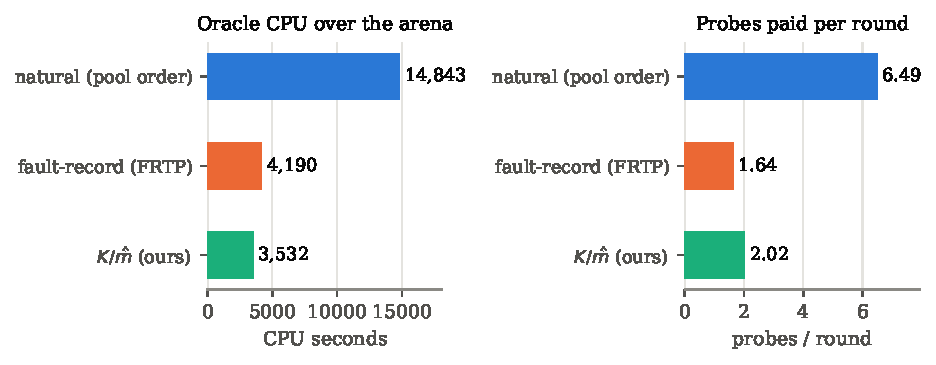
\includegraphics[width=\textwidth]{figures/fig-measured.pdf}
\caption{Measured oracle cost and probe count on the arena. The two panels
rank the policies in \emph{opposite} orders.}
\label{fig:measured}
\end{figure}

\paragraph{Reading.} Against the incumbent the result is large and
uncontroversial: \km\ removes $76.2\,\%$ of the oracle's CPU and is cheaper on
$63$ of $68$ tasks. The interesting comparison is against \frtp, and it is
interesting because the two units of account \textbf{disagree in sign}. \km\
pays $23.3\,\%$ \emph{more} probes and $15.7\,\%$ \emph{less} CPU. The
right-hand column of Table~\ref{tab:measured} shows the mechanism directly:
\frtp\ pays 0.3754\,s per probe --- \emph{more} than the incumbent's
0.3362\,s, because ranking on the kill count steers it towards
exactly the expensive cases that Table~\ref{tab:arena}'s last row predicts ---
while \km\ pays 0.2567\,s, $32\,\%$ less per probe. \km\ does not
find refutations in fewer steps; it finds them in cheaper steps.

This is the pilot's methodological contribution, and it is a caution rather
than a boast. \citet{lou2024aprregression} report executions rather than
seconds for a defensible reproducibility reason, and on a uniform-cost pool
that reporting choice is free. On this pool it would have inverted the
conclusion: measured in executions, \frtp\ wins by $23\,\%$.

\begin{figure}[H]
\centering
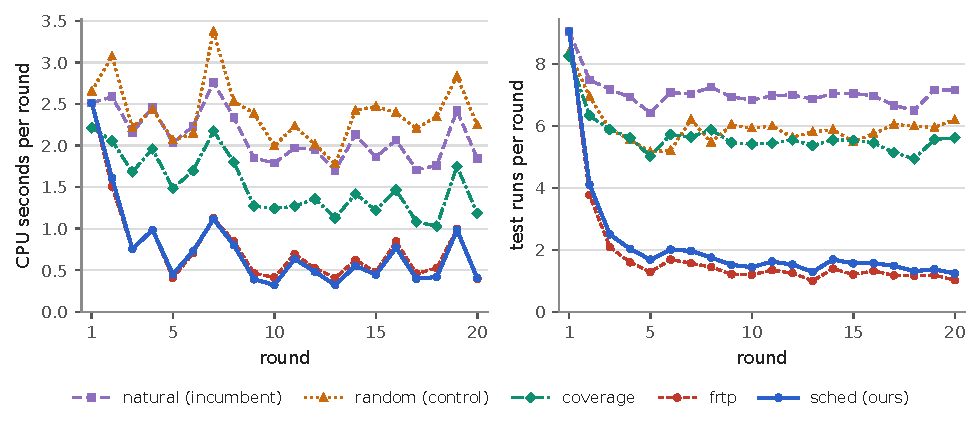
\includegraphics[width=0.72\textwidth]{figures/fig-round-curve.pdf}
\caption{Measured oracle CPU per round. The incumbent never learns; both
memories collapse within about three rounds; \km\ continues to separate from
\frtp\ as its cost model fills in.}
\label{fig:curve}
\end{figure}

Figure~\ref{fig:curve} shows that the ledger is doing what it is supposed to.
In round~1 every policy is identical by construction --- the ledger is empty,
so there is nothing to rank by --- and all three pay about 2\,s. By
round~5 both memory policies have collapsed to roughly a quarter of that. The
two then separate slowly: \frtp\ plateaus around 0.50\,s while \km\
continues down to 0.359\,s by round~20, because its cost estimates
keep improving while \frtp\ has nothing left to learn.

\begin{figure}[H]
\centering
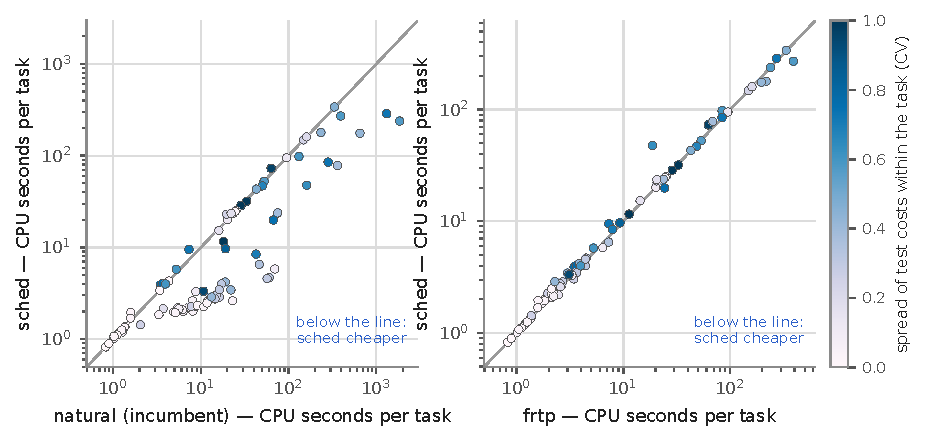
\includegraphics[width=0.52\textwidth]{figures/fig-per-task.pdf}
\caption{Per-task measured CPU, \km\ against \frtp. The win is broad rather
than driven by outliers, but it is not universal.}
\label{fig:pertask}
\end{figure}

Figure~\ref{fig:pertask} is the honest view of the \frtp\ comparison. \km\ is
cheaper on $42$ of $68$ tasks --- a clear majority, not a sweep --- and the
aggregate margin comes partly from the expensive tasks on the upper right,
where the cost spread inside the pool is largest. On cheap, homogeneous pools
the two policies are interchangeable, which is what the theory predicts.

\subsection{Replay Head-to-Head}
\label{sec:pilot-replay}

The replay study puts eight further policies on the same arena without paying
to execute them, by reconstructing from the complete verdict matrix exactly
what each would have probed. It uses $20$ seeds per task. Because the replay
reuses the measured per-case costs, it is a counterfactual over
\emph{orderings}, not a model of execution.

\begin{table}[H]
\centering
\caption{Replay over the arena, $20$ seeds. $\Delta$ is against plain \km;
CIs are a cluster bootstrap over the 68 tasks.}
\label{tab:replay}
\small
\begin{tabular}{@{}l r r r l c@{}}
\toprule
Policy & CPU (s) & probes/rd & $\Delta$ vs \km & 95\,\% CI & sig.\\
\midrule
\code{natural} (pool order)         & 18{,}297.1 & 6.375 & $+589.4\,\%$ & $[+216.8, +990.7]$ & $\star$\\
\code{random} (control)             & 13{,}275.8 & 4.252 & $+400.2\,\%$ & $[+232.6, +549.1]$ & $\star$\\
\code{coverage} ($\mathrm{RTP_{add}}$) & 16{,}611.3 & 5.368 & $+525.8\,\%$ & $[+192.1, +877.0]$ & $\star$\\
\code{cost-only} ($1/\hat m$)       & \phantom{0}8{,}810.6 & 5.083 & $+231.9\,\%$ & $[\phantom{0}+78.9, +403.1]$ & $\star$\\
\code{kill-only} ($K$)              & \phantom{0}2{,}800.9 & 1.305 & $\phantom{00}+5.5\,\%$ & $[\phantom{00}-7.3, \phantom{0}+23.6]$ & \\
\code{km} (\km)                     & \phantom{0}2{,}654.2 & 1.943 & \phantom{00}$0.0\,\%$ & --- & \\
\textbf{\kmc{0.5} (proposed)}       & \phantom{0}\textbf{2{,}409.4} & 1.474 & $\phantom{00}\bm{-9.2\,\%}$ & $[\phantom{0}-15.0, \phantom{00}-1.6]$ & $\bm\star$\\
$K^{0.5}g^{0.25}/\hat m^{0.25}$     & \phantom{0}2{,}366.4 & 1.500 & $\phantom{0}-10.8\,\%$ & $[\phantom{0}-16.1, \phantom{00}-4.2]$ & $\star$\\
\bottomrule
\end{tabular}
\end{table}

Three readings follow.

\emph{The memory term carries most of the effect.} Going from \code{natural} to
\code{kill-only} takes CPU from $18{,}297$ to $2{,}801$. That is the step that
matters most, and it is the step \frtp\ already takes --- which is why \frtp\
is the right baseline and \code{natural} is not.

\emph{Cost alone is not enough.} \code{cost-only} ranks by $1/\hat m$ with no
kill information and lands at $8{,}811$: better than pool order, far worse than
any policy that knows which cases refute. The two terms are not substitutes.

\emph{Additional-greedy coverage does not transfer.} The $\mathrm{RTP_{add}}$
arm reaches $16{,}611$, barely better than pool order and much worse than the
random control. Coverage of the \emph{reference} program is nearly constant
across a contest task's pool --- the median within-task coefficient of
variation of covered-line count is $0.073$ --- so there is almost no marginal
coverage to be greedy about. This is a negative result worth stating plainly:
the strongest classical prioritiser is useless in this setting.

\subsection{How Much to Divide by Cost}
\label{sec:pilot-sweep}

Equation~\eqref{eq:score} leaves the exponent $c$ free, and the two endpoints
are the two published positions: $c = 0$ is the \frtp\ family's kill-only
ranking and $c = 1$ is full cost-cognizance. The sweep measures it.

\begin{figure}[H]
\centering
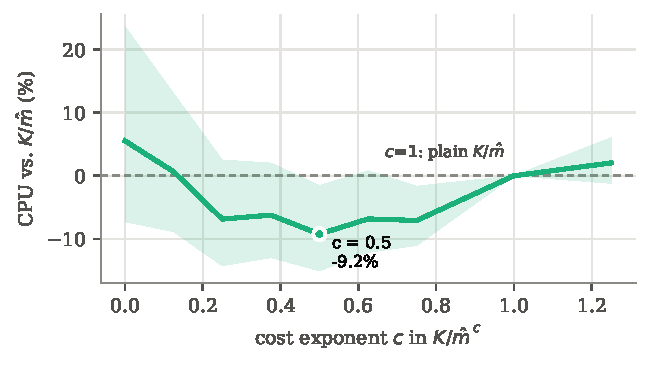
\includegraphics[width=0.72\textwidth]{figures/fig-c-sweep.pdf}
\caption{Cost-exponent sweep, $20$ seeds, paired per task. The optimum is
interior: dividing by cost helps, dividing by the \emph{full} cost
over-corrects.}
\label{fig:csweep}
\end{figure}

The curve is U-shaped with a minimum at $c = 0.5$, which beats plain \km\ by
$9.2\,\%$ (CI $[-15.0, -1.6]$). Both endpoints are worse: $c=0$ costs
$+5.5\,\%$ and $c=1.25$ costs $+2.0\,\%$, neither significantly different from
\km. The interpretation is that $\hat m$ is a noisy online estimate, and a
square root is the standard way to use a noisy denominator without letting one
cheap-looking early measurement dominate the ranking. The practical conclusion
for Phase~2 is that $c$ must be a tuned parameter with a declared default, not
a constant fixed at $1$ by the name of the method.

A companion sweep added the marginal-coverage term $g$ of
Equation~\eqref{eq:additional} as a third factor at fifteen $(a,b,c)$
combinations. Of the fifteen, twelve have confidence intervals straddling
zero; the largest effect at the operating point $a{=}1, c{=}0.5$ is
$-2.2\,\%$ with CI $[-5.0, +0.9]$. Coverage is therefore \textbf{dropped from
the proposed score}: it costs a tracing pass per case and buys nothing
measurable.

\subsection{Soundness Check}
\label{sec:soundness}

Definition~\ref{def:soundness} says no ordering can change which patches are
accepted. The measured runs confirm it: all three policies accepted exactly
$6$ patches over the $6{,}800$ rounds each. A discrepancy here would have been
a soundness bug rather than a finding, and the check is cheap enough to repeat
on every cell in Phase~2.

\subsection{Reproducibility}

Every number in this section is regenerated from three input files --- the
verdict matrix, the per-case cost table and the per-case coverage table ---
by the scripts shipped under \code{report/scripts/}. The replay head-to-head
and the exponent sweep were re-run from scratch for this document and
reproduce the stored values to the printed precision; the measured block is a
direct aggregation of the $33{,}000$-row round log. Generated artefacts are
under \code{report/data/}.

\section{Discussion}
\label{sec:pilot-discussion}

\paragraph{What the evidence supports.} Three claims are supported at the
pilot's scale. The oracle's cost in a counterexample-guided repair loop is
dominated by probe ordering, and a per-case memory removes about three quarters
of it. A cost-aware ranking beats the published kill-count ranking by a
further $15.7\,\%$ of CPU, with the margin coming from cheaper probes rather
than fewer ones. And the unit of account is not neutral on this corpus: CPU and
executions order the policies oppositely, so a prioritisation result reported
in executions alone does not transfer to a deployment that pays seconds.

\paragraph{What it does not support.} The pilot says nothing about the
proposer. RQ3 and RQ4 --- whether a counterexample keyed to a test case and
phrased as a positive requirement renormalises the patch distribution, and at
what disclosure that turns into fitting the shown tests --- are untouched,
because the \cegmem\ data was collected under a prohibition-style prompt and no
replay can manufacture a counterfactual model call. It also says nothing about
scale: $68$ tasks is a pilot, the arena is restricted to tasks whose cost and
coverage passes finished, and that restriction is not random with respect to
task cost. Finally, the $15.7\,\%$ margin over \frtp\ has a wide interval
($[-28.9, -5.1]$) and holds on $42$ of $68$ tasks; it is a real effect at this
scale, not a settled magnitude.

\paragraph{Threats carried into Phase 2.} Three are worth naming now. The
arena's selection is cost-correlated, so the full corpus may show a smaller
margin. The replay reuses one cost measurement per case rather than sampling
the cost distribution, which understates variance --- the measured block exists
precisely so the headline does not depend on the replay. And \code{gpt-4o-mini}
produced every patch in the matrix, so the patch population, and therefore the
kill structure the ledger learns, is one model's.
